\chapter{Components}

The logical components are the building blocks of the system. They usually
manifest through a namespace or a directory structure, where leaf nodes
containing source code represent the logical components.


\begin{itemize}
  \item[] \textbf{Logical architecture}: the system's logical components and how they
        interact each other.
  \item[] \textbf{Physical architecture}: includes also physical artifacts, defining architectural
\end{itemize}

\section{Identify components}


\begin{center}
  \centering
  \begin{minipage}{1\linewidth}
    % Primo blocco: 50% dello spazio per il codice
    \begin{minipage}{0.65\linewidth}
      \paragraph{Example: } SPG = Solidarity Purchasing Group,
      Solidarity towards producers valuing (small vs large, local
      and seasonal vs global and specific vs mass).

      Solidarity among clients: Not a normal shop but a group of people buying together,
      sharing the principles to select producers.

      This is a software application for \textbf{Clients}, \textbf{Farmers} and \textbf{Shop employees}.

    \end{minipage}% <-- IMPORTANTE: il simbolo % qui evita spazi bianchi extra
    \hfill
    \begin{minipage}{0.3\linewidth}
      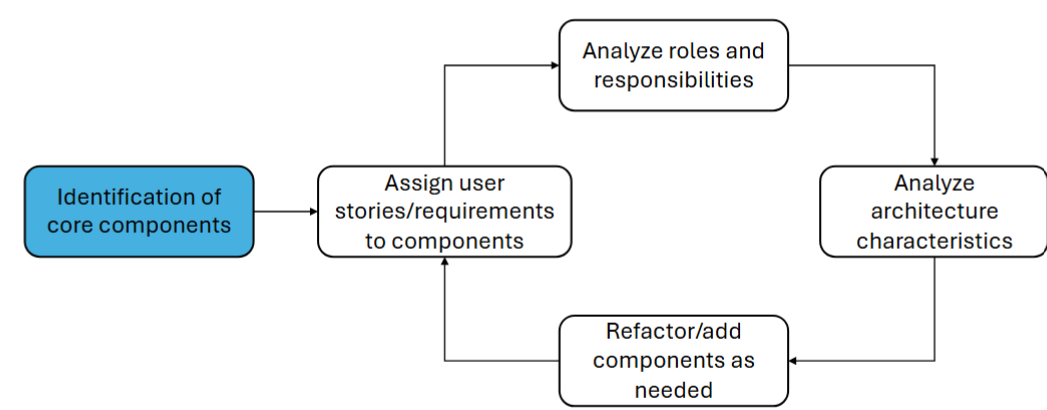
\includegraphics[width=1\linewidth]{images/Components/C-esempio1.png}
    \end{minipage}
  \end{minipage}
\end{center}

The identification of components is fundamental activity, necessary either for
drafting architecture from scratch or reverse-engineer it.
It is an iterative refinement process and three approaches can be used for
initial identification:

\begin{itemize}
  \item \textbf{Best guess}: based on the system core functionalities
  \item \textbf{Workflow}: Based on the "happy path"
  \item \textbf{Actor/action}: Based on major actions a user can perform
\end{itemize}


\subsubsection{SPG requirements}

A neighborhood association manages a Solidarity Purchasing Group
(SPG). Every Monday, a farm (rotating among a pool of reference
suppliers) submits to the SPG a list of available products, their
quantities, and their prices.\newline

Once this list is provided, the data is reviewed and confirmed by the
SPG employee.\newline

SPG members receive an email with the list of available products and
can place their orders either via the website or by visiting the
association's headquarters.\newline

When ordering, SPG members specify the types of vegetables they
want and the quantities (expressed in kilos, packs, or boxes
depending on the type of fruit or vegetable ordered). If the order is
placed at the association's headquarters, the member pays
immediately.\newline

At the end of the week, the farm delivers the products to the
association's headquarters. Shop employees record the delivery, and
members receive a notification when their ordered goods arrive. At
this point, members can go to the association to collect the package
(paying at the same time, if not done at the time of ordering).


\begin{table}[htbp]
  \renewcommand{\arraystretch}{1.5}
  \centering
  \begin{tabular}{ll}
    \textbf{Macro functionality} & \textbf{Component} \\

    \hline
    Insert products              & Product submission \\
    View products                & Product browser    \\
    Order products               & Order placement    \\
    Buy products                 & Order Payment      \\
  \end{tabular}
\end{table}


\subsubsection{Workflow approach}

\begin{table}[htbp]
  \renewcommand{\arraystretch}{1.5}
  \centering
  \begin{tabular}{ll}
    \textbf{Step}                                          & \textbf{Component}  \\

    \hline
    1. Farmer submits available products, employee reviews & Product submission  \\
    2. SPG members/clients receive list of products        & Client notification \\
    3. Client browse the catalog of product                & Product browser     \\
    4. Client places an order                              & Order placement     \\
    4a. Employee places an order for the client            & Order placement     \\
    5. Client pays the order online                        & Order Payment       \\
    5a. Employee submit order payment                      & Order Payment       \\
    6. Employees register delivery of goods                & Product delivery    \\
    7. Clients are updated on goods' delivery              & Client notification \\
    8. Clients retrieve goods                              & Product delivery    \\
  \end{tabular}
\end{table}


\subsubsection{Actor/action}


\begin{table}[hbt!]
  \centering
  \renewcommand{\arraystretch}{1.5}% Aumenta leggermente l'altezza delle righe per una migliore leggibilità
  \begin{tabular}{llll}
    \textbf{Actor}                 & \textbf{Action}                & \textbf{Component} \\ \hline
    \multirow{4}{*}{Client}        & Search for products            & Product browser    \\
                                   & View details about products    & Product browser    \\
                                   & Place order                    & Order placement    \\
                                   & Pay order                      & Order payment      \\ \hline
    Farmer                         & Insert products availabilities & Product submission \\ \hline
    \multirow{4}{*}{Shop employee} & Review products availabilities & Product review     \\
                                   & Insert client order            & Delegate order     \\
                                   & Insert client payment          & Delegate payment   \\
                                   & Register product delivery      & Order delivery     \\ \hline
    System !                       & Send email notifications       & Email Notification \\
  \end{tabular}
\end{table}


\begin{figure}[h!]
  \centering
  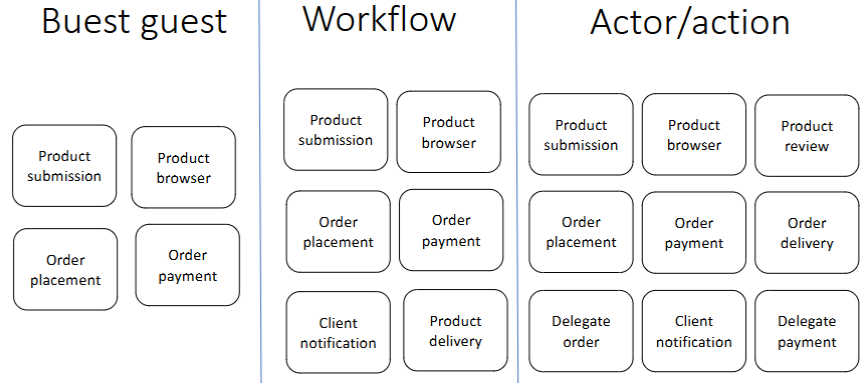
\includegraphics[width=0.35\linewidth]{images/Components/C-esempio7.png}
\end{figure}

\subsection{Putting components together}

\begin{itemize}
  \item \textbf{Tactic level - design}: Components principles: cohesion, coupling
  \item \textbf{Strategic level - architecture}: Component topology, technical partitioning vs domain partitioning, and Physical architecture, Monolithic vs Distributed architecture.
  \item \textbf{And more}: Deployment, communication style and data topology
\end{itemize}

\section{Component principles}

\subsection{Component cohesion}

How to put classes inside a component?

Cohesion is the degree to which the
classes within a component belong together.

\textbf{High cohesion} means that the
classes within a component are closely related in terms of functionality
and purpose, while \textbf{low cohesion} indicates that the classes are more unrelated
and serve different purposes.


It is suggested to follow principle:

\begin{itemize}
  \item The \textbf{Reuse/Release Equivalence Principle - REP}: The granule of reuse is the granule of release.
  \item The \textbf{Common Closure Principle - CCP}: Classes that change together are packaged together.
  \item The \textbf{Common Reuse Principle - CRP}: Classes that are used together are packaged together.
\end{itemize}

\subsubsection{Reuse/Release Equivalence Principle - REP}
To support reuse, classes and modules that make up a component
must: belong to a coherent group and be released together.

The release process shall produce appropriate notifications and release
documentation, so that users can decide whether to integrate new releases.


\subsubsection{Common Closure Principle - CCP}
Group into components classes that change together, i.e. for the same
reason and at the same time.


Separate into different components classes that have different
changes processes and motivation.


\begin{tcolorbox}
  \textbf{Note:} There is a relationship between the Common Closure Principle (CCP).  It is similar to SRP and it addresses the "closure" aspect of OCP
\end{tcolorbox}


\begin{flushleft}
  \begin{minipage}{0.65\linewidth}
    \raggedright
    \subsubsection{Common Reuse Principle - CRP}

    It help deciding which classes/module to place into the same
    components. In such components, usually classes have many dependencies on
    each other

    Complementary perspective:

    \begin{itemize}
      \item users of a component should not depend on unnecessary features;
      \item if a class isn't closely connected to another class, it shouldn't be in
            the same component.
    \end{itemize}

    Similar to interface segregation design principle (ISP).

  \end{minipage}%
  \hfill
  \begin{minipage}{0.3\linewidth}
    \centering
    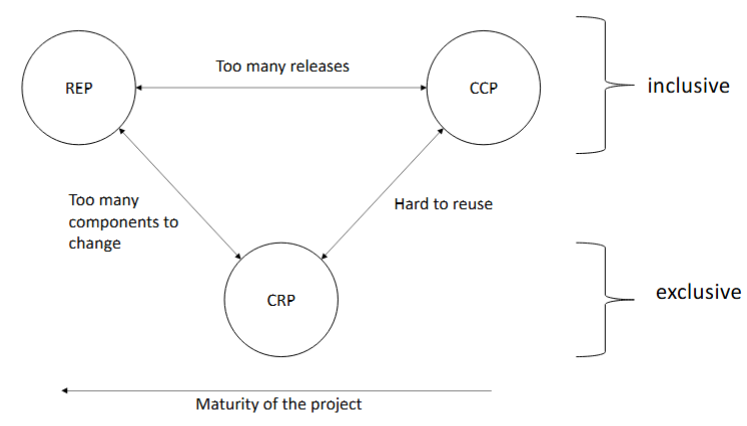
\includegraphics[width=\linewidth]{images/Components/C-esempio2.png}
  \end{minipage}
\end{flushleft}

\begin{tcolorbox}
  \textbf{Note:} Similar to interface segregation design principle (ISP)
\end{tcolorbox}


\subsection{Component coupling}

\begin{itemize}
  \item The Acyclic Dependencies Principle (ADP): The dependency graph of packages must have no cycles.
  \item The Stable Dependencies Principle (SDP): Depend in the direction of stability.
  \item The Stable Abstractions Principle (SAP): Abstractness increases with stability.
\end{itemize}


\subsubsection{Acyclic Dependencies Principle - ADP}

Historical roots on typical issues of team-based development: the \textit{morning after syndrome}\footnote{The morning after syndrome occurs when code worked on, tested, and left working one day is broken the next morning due to changes made by others} and the \textit{weekly build}.

\begin{center}
  \begin{minipage}{0.65\linewidth}

    Solution to the problem: partition the development environment into
    releasable components


    Each component has its own responsible developer/team so the
    releases are uniquely identified and components follow their own, private, development path.
    E.g. in git versioning system, using separated branches or even separated repositories.

  \end{minipage}%
  \hfill
  \begin{minipage}{0.3\linewidth}
    \centering
    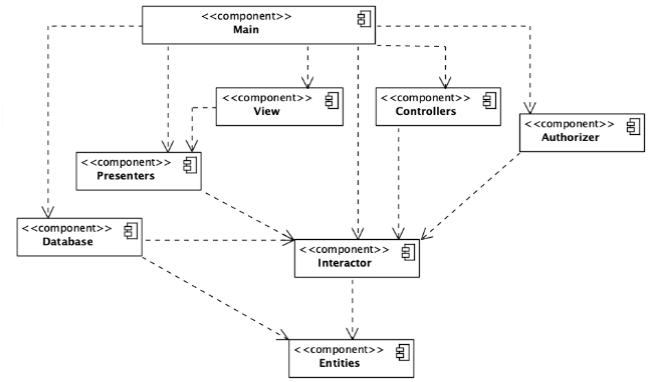
\includegraphics[width=\linewidth]{images/Components/C-esempio8.png}

  \end{minipage}
\end{center}


\begin{itemize}
  \item \textbf{Advantages}: Changes made to one component do not affect other
        teams, until they decide to adapt to the new component's release. I
        ntegration happens in small steps
  \item \textbf{Implications}: teams must monitor, manage and, maintain the
        dependency structure over time. there can be no "cycles" or circular
        dependencies in the dependency graph.
\end{itemize}

\paragraph{Example: directed acyclic graph}

Starting at any component, it is not possible to get back to the origin by
following the edges (dependencies).


What happens when a change is made to Presenters?
View and Main will be affected and tests with
Interactor and Entities.

The bottom-up "building" for system release

\begin{itemize}
  \item Entities
  \item Database and Interactor
  \item Presenters, View, Controllers, Authorizer
  \item Main
\end{itemize}

\paragraph{Example 2: dependency cycle}

Now imagine a new dependency arises: User class in Entities uses the Permissions
class in Authorizer.

Testing Entities requires now also Authorizer and Interactor.

There are different ways to solve this problem:

\begin{itemize}
  \item Solution A: Use dependency inversion principle (DIP)
  \item Solution B: Create a new component on which both Entities and
        Authorizer depend. Move the class(es) they both depend on into this new
        component.

\end{itemize}


\subsection{The Stable Dependencies Principle - SDP}

Depend in the direction of stability.
Stability is not about the frequency of changes, but about the amount of work
required to make a change.

A cupboard is stable because it takes a lot of effort to move it,
while a cup is not stable because it takes little effort to move it.



A component with lots of incoming dependencies is very stable because it
requires a great deal of work to reconcile any changes with all the dependent
components.

Modules that are designed to be harder to modify should not depend on modules
that require little effort to change.


\subsubsection{A simple measure of (in)stability}

X is very stable because three components depend on it and it
depends on no other component, while Y is very unstable because
no component depends on it and it depends on three other components.

\begin{flushleft}
  \begin{minipage}{0.65\linewidth}
    \raggedright
    \textbf{Instability: } goes from 0 to 1, where 0 is the most stable and 1 is the most unstable.

    \begin{equation*}
      \centering
      I = \frac{\text{Fan-out}}{\text{Fan-in + Fan-out}}
    \end{equation*}

    \vspace{0.75cm}
    Where

    \begin{itemize}
      \item Fan-in is the number of incoming dependencies
      \item Fan-out is the number of outgoing dependencies
    \end{itemize}
  \end{minipage}%
  \hfill
  \begin{minipage}{0.3\linewidth}
    \centering
    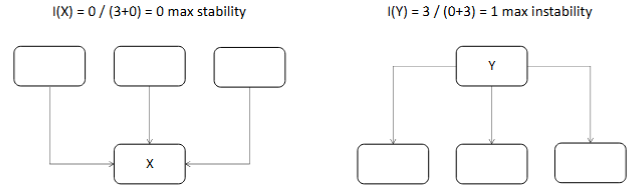
\includegraphics[width=\linewidth]{images/Components/C-esempio3.png}
  \end{minipage}
\end{flushleft}



\paragraph{Example: } I(C\_B) = 0.33. Fan-in = 4 and Fan-out = 2. I(C\_D) = $\frac{2}{4+2} = 0.33$.


\begin{figure}[h!]
  \centering
  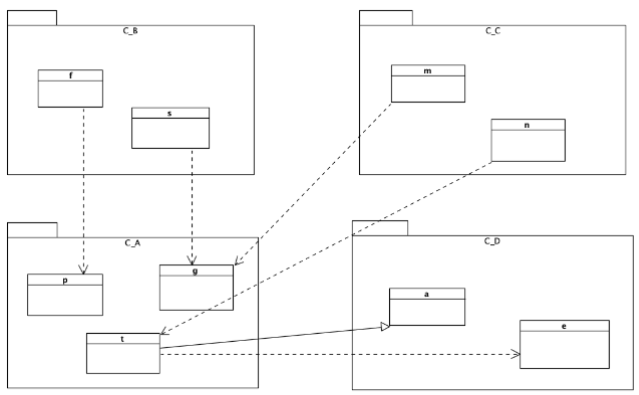
\includegraphics[width=0.35\linewidth]{images/Components/C-esempio9.png}
\end{figure}

\subsubsection{SDP and stability measure}

Depend in the direction of stability.

The I(component) should be larger than the I(the components that it depends on).
I metric should decrease in the direction of dependency.
$I(C_B) = I(C_C) > I(C_A) > I(C_D)$


\paragraph{SDP violation as system evolves: example}

Requirements: C should be stable. D should be flexible.

\begin{figure}[h!]
  \centering
  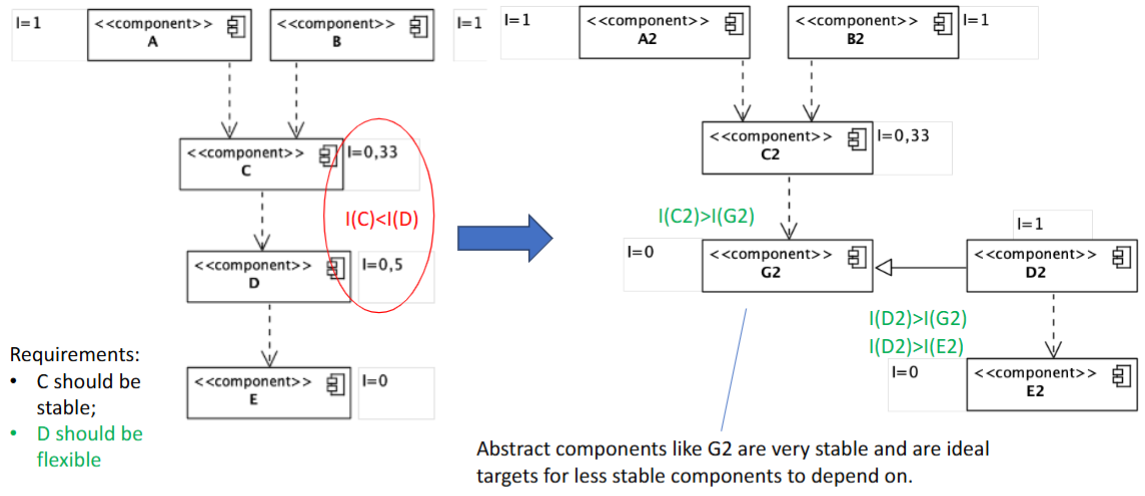
\includegraphics[width=0.45\linewidth]{images/Components/C-esempio10.png}
\end{figure}


\subsection{Stable Abstractions Principle - SAP}

A component should be as abstract as it is stable. Code that represent
high-level policies of the system should be placed into stable components.


\subsubsection{SAP, OCP, SDP and abstract classes}
Open Closed principle suggests creating classes that are flexible enough to be
extended without requiring modification. Abstract classes are best suited to
this need. Thus, applying SDP: stability goes into the direction of abstraction



\begin{flushleft}
  \begin{minipage}{0.65\linewidth}
    \raggedright

    \paragraph{A simple measure of abstractness this ratio:}


    \begin{equation*}
      \centering
      A = \frac{\text{Number of abstract classes and interfaces in the component}}{\text{Total number of classes in the component}}
    \end{equation*}


    \vspace{0.75cm}
    where:
    \begin{itemize}
      \item A = 0 means that the component is completely concrete. No abstract classes.
      \item A = 1 means that the component is completely abstract. Only abstract classes.
    \end{itemize}
  \end{minipage}%
  \hfill
  \begin{minipage}{0.3\linewidth}
    \centering
    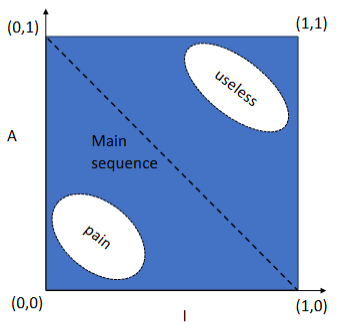
\includegraphics[width=\linewidth]{images/Components/C-esempio5.png}
  \end{minipage}
\end{flushleft}


\begin{tcolorbox}
  \textbf{Note:} Distance from the main sequence: $D = |A + I - 1|$
\end{tcolorbox}




\section{Strategic decisions}

\subsection{Iterative Refinement}

\begin{center}
  \begin{minipage}{0.47\linewidth}
    \centering
    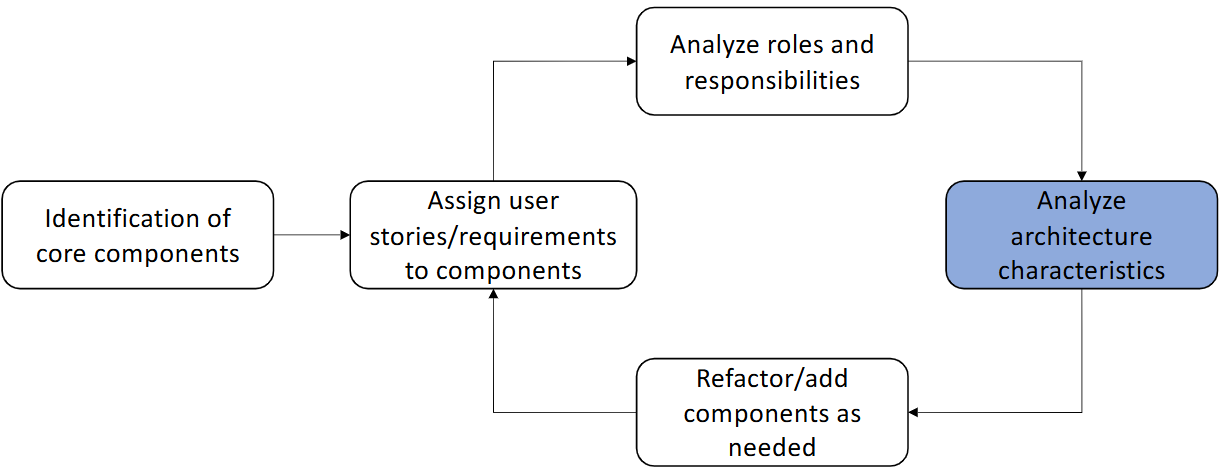
\includegraphics[width=\linewidth]{content/chapters/images/2026-03-22-10-17-17.png}
  \end{minipage}%
  \hfill
  \begin{minipage}{0.47\linewidth}
    \centering
    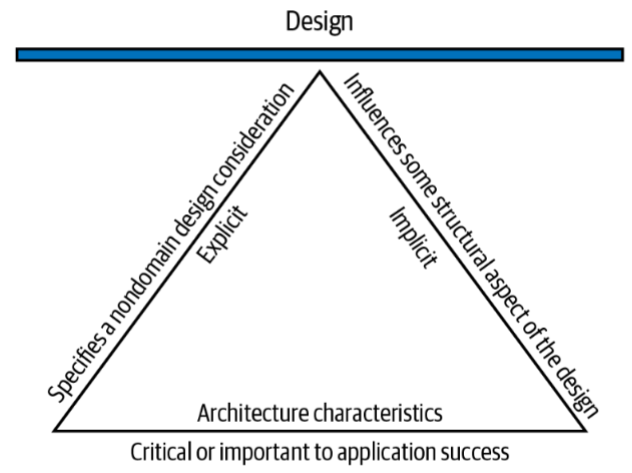
\includegraphics[width=0.55\linewidth]{content/chapters/images/2026-03-22-10-18-26.png}
  \end{minipage}
\end{center}


\subsubsection{Operational Architectural Characteristics: examples}

\begin{itemize}
  \item \textbf{Scalability}: the system's ability to perform and operate as the number
        of users or requests increases
  \item \textbf{Elasticity}: the system's ability to perform and operate with peaks of
        requests
  \item \textbf{Responsiveness}: the system's ability to complete assigned tasks
        within a given time
  \item  \textbf{Reliability/safety}: Whether the system needs to be fail-safe, or if it is
        mission critical in a way that affects lives. Fault tolerance does the software operate as intended despite hardware or
        software faults.
  \item \textbf{Availability}: How much of the time the system will need to be
        available; if that's 24/7, steps need to be in place to allow the system to be
        up and running quickly in case of any failure.
  \item \textbf{Continuity}: The system's disaster recovery capability.
  \item \textbf{Robustness}: The system's ability to handle error and boundary conditions
        while running, for example, if the internet connection or power fails.
  \item ...
\end{itemize}


\subsubsection{Engineering Architectural Characteristics}

\begin{itemize}
  \item \textbf{Maintainability}: the degree of effectiveness and efficiency to which
        developers can modify the software to improve it, correct it, or adapt it to
        changes in environment and/or requirements.
  \item \textbf{Testablity}: how easily developers and others can test the software?
        How complete are tests?
  \item \textbf{Deployability}: ease, frequency and overall risk of deployment
  \item \textbf{Evolvability}: system's ability to survive changes in its environment,
        requirements and implementation technologies
  \item ...
\end{itemize}

\begin{center}
  \begin{minipage}{0.65\linewidth}

    \subsection{Strategic level: partitioning}
    Technical partitioning vs domain partitioning

  \end{minipage}%
  \hfill
  \begin{minipage}{0.3\linewidth}
    \centering
    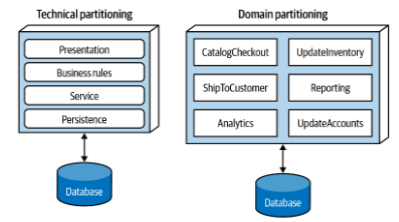
\includegraphics[width=\linewidth]{content/chapters/images/2026-03-22-10-38-08.png}
  \end{minipage}
\end{center}



\subsection{Conway's law}

Organizations which design systems...are constrained to produce
designs which are copies of the communication structures of these
organizations.


The structure of the design will reflect how people communicate
and work together


\subsection{Monolithic versus Distributed architecture}

\begin{itemize}
  \item[]  \textbf{Monolithic}: single deployment unit of all code
  \item[] \textbf{Distributed}: multiple deployment units connected through remote
        access protocols
\end{itemize}


\begin{table}[htbp]
  \renewcommand{\arraystretch}{1.5}
  \centering
  \begin{tabular}{ll}
    \textbf{Monolithic}   & \textbf{Distributed} \\
    \hline
    Layered architecture  & Service-based        \\
    Pipeline architecture & Event-driven         \\
    Modular monolith      & Space-based          \\
    Microkernel           & Service-oriented     \\
                          & Microservices        \\
  \end{tabular}
\end{table}

